
%(BEGIN_QUESTION)
% Copyright 2010, Tony R. Kuphaldt, released under the Creative Commons Attribution License (v 1.0)
% This means you may do almost anything with this work of mine, so long as you give me proper credit

A DDC (Direct Digital Control) system used for building automation sends a 4-20 mA control signal to a steam valve with an electronic positioner.  This particular loop has a problem, for the valve remains in the full-closed (0\%) position regardless of what the DDC tries to tell it to do.  A technician begins diagnosing the problem by taking a DC voltage measurement at terminal block TB-11 in this loop circuit:

$$\includegraphics[width=15.5cm]{i04239x01.eps}$$

The technician knows a reading of 0 volts could indicate either an ``open'' fault or a ``shorted'' fault in the wiring.  Based on the location of the measured voltage (0.00 VDC), determine where in the wiring a single ``open'' fault would be located (if that is the culprit), and also where in the wiring a ``short'' fault would be located (if that is the culprit).

\vskip 10pt

For the next diagnostic test, the technician disconnects the red wire of cable 30 where it attaches to the screw terminal on TB-11, and re-measures voltage at TB-11.  After disconnecting the wire, the new voltage measurement at TB-11 reads 25.3 volts.  Determine what this result tells us about the nature and location of the fault.

\vskip 20pt \vbox{\hrule \hbox{\strut \vrule{} {\bf Suggestions for Socratic discussion} \vrule} \hrule}

\begin{itemize}
\item{} Explain why it is critically important to determine the identities of the valve and DDC card as being either electrical {\it sources} or electrical {\it loads} when interpreting the diagnostic voltage measurements.
\item{} Identify some of the pros and cons of this style of testing (measuring voltage at a set of points before and after a purposeful wiring break) compared to other forms of multimeter testing when looking for either an ``open'' or a ``shorted'' wiring fault.
\item{} Identify a fault other than open or shorted cables which could account for all the symptoms and measurements we see in this troubleshooting scenario.
\end{itemize}

\underbar{file i04239}
%(END_QUESTION)





%(BEGIN_ANSWER)

Based on the first measurement (only), we could conclude the wiring fault {\it may} be an ``open'' in cable 26, or a ``short'' in {\it any} cable. 

%(END_ANSWER)





%(BEGIN_NOTES)

After taking the second measurement, we must conclude the fault is a ``short'' (not an ``open''), and that it lies somewhere between TB-11 and the control valve.








\vskip 20pt \vbox{\hrule \hbox{\strut \vrule{} {\bf Virtual Troubleshooting} \vrule} \hrule}

This question is a good candidate for a ``Virtual Troubleshooting'' exercise.  Presenting the diagram to students, you first imagine in your own mind a particular fault in the system.  Then, you present one or more symptoms of that fault (something noticeable by an operator or other user of the system).  Students then propose various diagnostic tests to perform on this system to identify the nature and location of the fault, as though they were technicians trying to troubleshoot the problem.  Your job is to tell them what the result(s) would be for each of the proposed diagnostic tests, documenting those results where all the students can see.

During and after the exercise, it is good to ask students follow-up questions such as:

\begin{itemize}
\item{} What does the result of the last diagnostic test tell you about the fault?
\item{} Suppose the results of the last diagnostic test were different.  What then would that result tell you about the fault?
\item{} Is the last diagnostic test the best one we could do?
\item{} What would be the ideal order of tests, to diagnose the problem in as few steps as possible?
\end{itemize}


%INDEX% Troubleshooting review: electric circuits

%(END_NOTES)


